\documentclass[tikz,border=5pt]{standalone}
\usepackage{pgfplots}
\usepackage{amsmath}
\pgfplotsset{compat=1.18}

\definecolor{corba}{HTML}{365FB3}
\definecolor{punt}{HTML}{B91C1C}
\definecolor{guia}{HTML}{6B7280}

\begin{document}
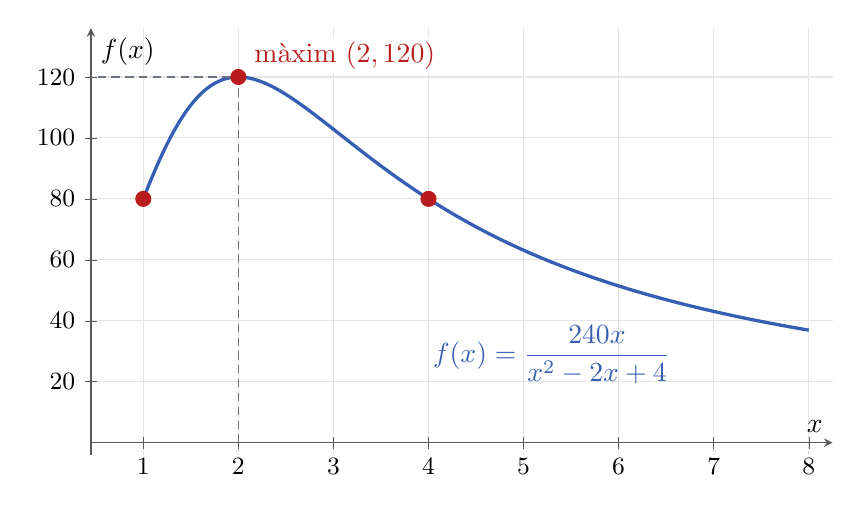
\begin{tikzpicture}
  \begin{axis}[
    width=11cm,
    height=7cm,
    axis lines=middle,
    xmin=0.45,
    xmax=8.25,
    ymin=-4,
    ymax=136,
    xlabel={$x$},
    ylabel={$f(x)$},
    xtick={1,2,3,4,5,6,7,8},
    ytick={0,20,40,60,80,100,120},
    grid=major,
    grid style={black!10},
    axis line style={black!65},
    tick style={black!65},
    tick label style={font=\small},
    clip=false,
  ]
    \addplot[corba, very thick, domain=1:8, samples=240]
      {240*x/(x^2-2*x+4)};

    \draw[guia, densely dashed]
      (axis cs:2,0) -- (axis cs:2,120) -- (axis cs:0.45,120);

    \addplot[only marks, mark=*, mark size=2.7pt, punt]
      coordinates {(1,80) (2,120) (4,80)};

    \node[anchor=south west, text=punt, fill=white, inner sep=1.5pt]
      at (axis cs:2.12,121) {màxim $(2,120)$};
    \node[anchor=north west, text=corba, inner sep=1.5pt]
      at (axis cs:4,40) {$f(x)=\dfrac{240x}{x^2-2x+4}$};
  \end{axis}
\end{tikzpicture}
\end{document}
